%!TEX root = ../report.tex
\chapter{Methodology}


\subsection{Formalization of Dynamic Motion Primitives}

\par Dynamic motion primitives use nonlinear differential equations to model the motion primitives. These differential equations is essentially represent a damped mass spring system. Attractor landscape of differential equations represent desired kinematic state of the robot. Over the time, various versions of DMPs were presented which were slightly different than one another, modified for specific use case or scenario. Following formalization of DMP is taken from \cite{ijspeert2013dynamical}.
A DMP can be represented by following set of equations,  
\begin{equation}\label{DMP_1}
\tau\dot{z} = \alpha_{z}(\beta_{z}(g - y) - z) + f(x)
\end{equation}
\begin{equation}\label{DMP_2}
\tau \dot{y} = z
\end{equation}
and the non-linear function $f(x)$
\begin{equation}\label{forcing_term}
f(x) = \frac{\sum_{i=1}^{N}\psi_{i}(x)w_{i}}{\sum_{i=1}^{N}\psi_{i}(x)}x(g - y_{0})
\end{equation}
where,
\begin{equation}\label{psi}
\psi_{i} = \exp(-{\frac{1}{2\sigma_{i}^{2}}(x - c_{i})^{2}})
\end{equation}
and,
\begin{equation}\label{canonical}
\tau \dot{x} = -\alpha_{x}x
\end{equation}
Equation \ref{DMP_1} and \ref{DMP_2} are the first order representation of a autonomous non-linear second-order differential equation where $f(x)$ is the non-linear term. 
Upon solving these equations, we get state $[\ddot{y}, \dot{y}, y]$ at each time instance. This state represents the acceleration, velocity and position i.e. kinematic state of robotic system. 

If the forcing term in eq. \ref{DMP_1} is made 0 i.e. $f = 0$, these equations represent a globally stable second-order linear system with $(z, y) = (0, g)$ as a unique point attractor. With appropriate value for $\alpha$ and $\beta$ (with $\beta_{z} = \alpha{z}/4$), the system can be made critically damped resulting in $y$ monotonically and asymptotically converging towards $g$. Such a system implements a stable but trivial pattern generator with $g$ as single point attractor \cite{ijspeert2013dynamical}.

By introducing term $f$, the path followed by the system in attractor landscape of differential equation from initial state to the goal state can be modified. This in turn modifies the trajectory followed by mobile robot or robotic manipulator in task-space or joint-space. This non-linear forcing function enables DMP framework to learn almost any arbitrary motion in end-effector space or joint space. It is essentially a weighted sum of equally spaced Gaussian functions denoted by $\psi$ (eq. \ref{psi}) activated at each time step by phase variable $x$. Forcing term $f(x)$ is learned from the demonstrated trajectories. It should be noted that the forcing term $f$ is modified by separation between goal and initial position ($g - y_{0}$), which ensures that the shape of trajectory is also modified by goal separation. Eq. \ref{DMP_1} and \ref{DMP_2} are together called \textit{transformation system}, as they transform current state of the system to next state.   

Equation \ref{canonical} is called \textit{canonical system}. $x$ acts as the phase variable modifying forcing term $f(x)$ and hence the shape of the trajectory. It removes the the explicit time dependency of of the system, which eliminates the need of maintaining complex timing mechanisms to synchronize multiple DMPs. $x$ initialized at 1 decays to 0 at the end of the motion ensuring convergence to goal state $g$. It is used to localize the basis functions (i.e., as a phase signal) but also provides an amplitude signal (or a gating term) that ensures that the nonlinearity introduced by the forcing term remains transient due to asymptotical convergence of $x$ to zero at the end of the discrete movement \cite{ijspeert2013dynamical}.

Term $\tau$ is time scaling factor which can be used to modify the speed of execution of the system by modifying the acceleration and velocity term.  

Similar to the above discussed point attractor behavior, DMPs can also learn rhythmic motions exploiting the limit cyclic behavior of non-linear second order differential equation. To achieve rhythmic motion, we need to learn forcing term $f(x)$ which is periodic itself and makes system of equation \ref{DMP_1} and \ref{DMP_2} exhibit limit cyclic behavior. This can be achieved by choosing canonical system to be,

\begin{equation}
	\tau \dot{\phi} = 1
\end{equation}  

where $\phi \in [0, 2\pi]$ is the phase angle of the oscillator in polar coordinates and the amplitude of the oscillation is assumed to be r. Similar to the discrete system, this rhythmic canonical system serves to provide both an amplitude signal $r$ and a phase signal $\phi$ to the forcing term $f$ in equation \ref{DMP_1}.

\begin{equation}
	f(r, \phi) = \frac{\sum_{i=1}^{N}\psi_{i}(x)w_{i}}{\sum_{i=1}^{N}\psi_{i}(x)}r
\end{equation}

\par Point attractor and limit cycle behaviors exhibited by non-linear second order differential equation can be used to model discrete (point to point) and rhythmic motions of robotic arm or mobile platform.   
\vspace{0.5cm}

During this Research and Development project, point attractor DMPs for discrete motion (point-to-point motion) were implemented. For the ease of implementation, above system was slightly modified as follows, 
\begin{equation}\label{actual_DMP}
	\ddot{y} = \tau^{2}\alpha_{y}(\beta_{y}(g-y)-\dot{y}) + f
\end{equation}
\begin{equation}
	\dot{x} = \tau(-\alpha_{x}x)
\end{equation}

This modification does'nt change the properties of original DMP formulation.


\begin{figure}[H]
	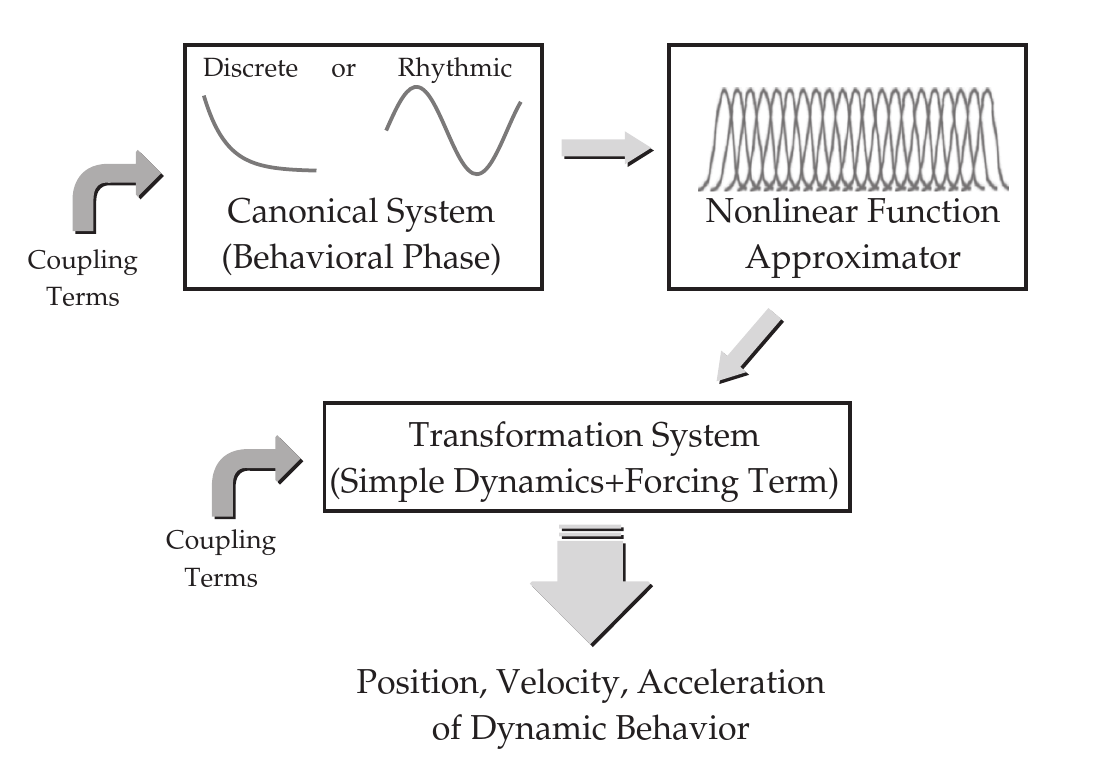
\includegraphics[width=\textwidth]{images/dmp.png}
	\caption{Dynamic Movement Primitive framework \cite{ijspeert2013dynamical}}
	\label{fig:DMP_framework}
\end{figure}
Figure \ref{fig:DMP_framework} taken from \cite{ijspeert2013dynamical} show composition of the DMP framework. The \textit{Coupling Terms} in the figure denotes consists of feedback form the sensors, obstacle coupling terms, error in execution speed of the DMPs. Canonical system generates the phase variable $x$ at each time step which is used for generating a non-linear forcing term. This forcing term then modifies the behavior of the kinematic motion commands generated by transformation system. Kinematic motion commands are then executed by robot controller (e.g. velocity controllers, torque controllers, etc.)

Figure \ref{fig:DMP_2DOF} shows the path generated by 2 degrees-of-freedom DMP with no forcing term in Cartesian space. Figure illustrates the superposition of 2 DMPs in different degrees of freedom. DMP systems in $X$ and $Y$ axes follow the kinematic trajectories same as of damped mass-spring system and superposition of these two motion generate a straight line motion in 2D space. 




\begin{figure}[H]
	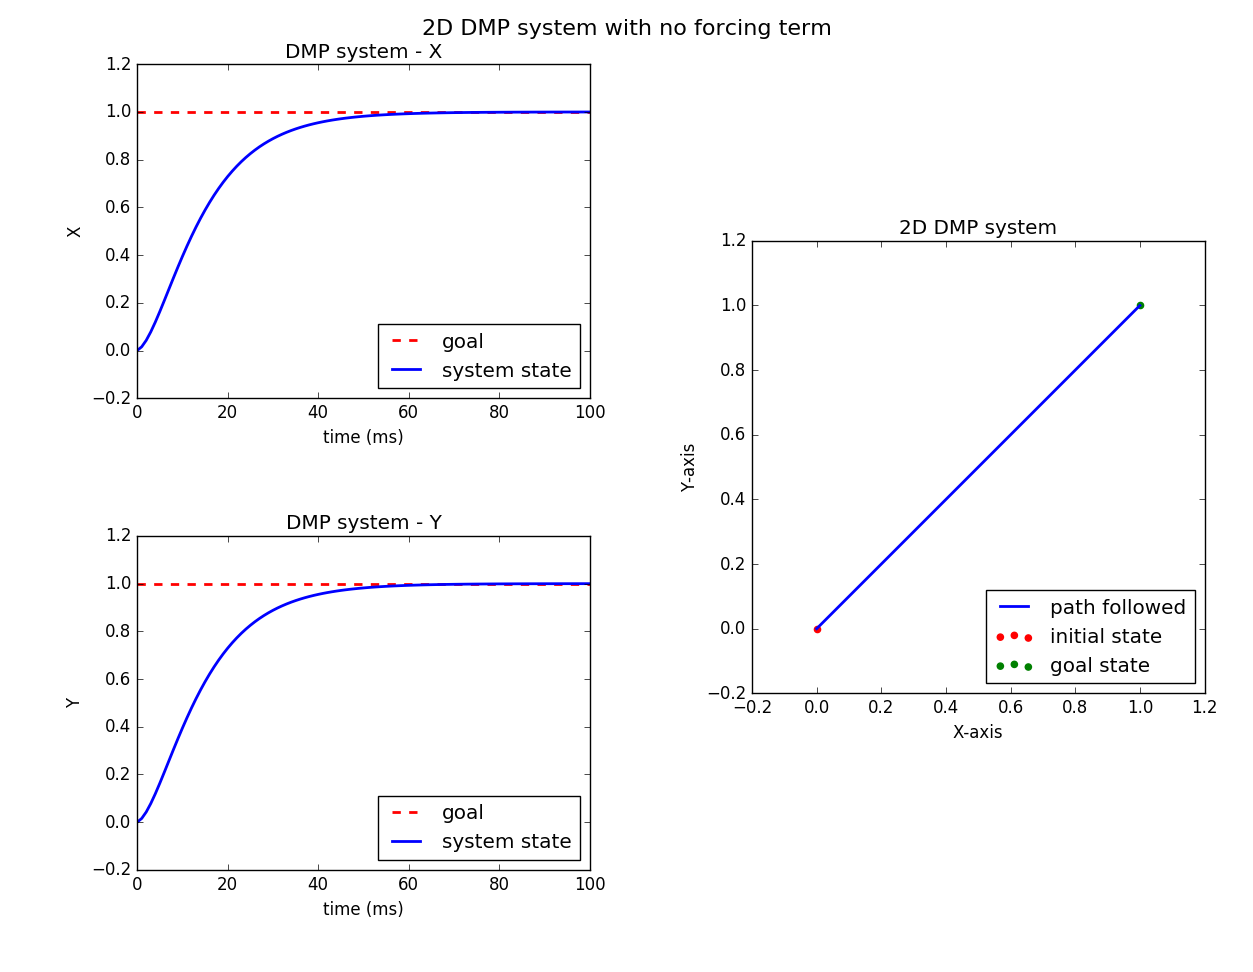
\includegraphics[width=\textwidth]{images/dmp_no_f.png}
	\caption{2D DMP with no forcing term}
	\label{fig:DMP_2DOF}
\end{figure}


\newpage

\subsection{Analysis of the effects of parameters used in DMP}

For analyzing the effects of the various parameters used in DMP, a artificially generated step function trajectory was learned. Parameters were changed in order to evaluate their effects on the DMP. The evaluation criteria was the closeness between the desired path and the path generated by DMP after learning. The error between path was calculated as normalized point-to-point distance between discrete positions on two paths. Error was calculated as follows:

\begin{equation}
	error = \frac{1}{N}\sum_{i = 1}^{N}min\{\norm{P_{i} - Pd_{1}}, \norm{P_{i} - Pd_{2}}, \norm{P_{i} - Pd_{3}}, .... , \norm{P_{i} - Pd_{M}}\}
\end{equation}

This error function evaluates the closeness of two paths, hence does'nt consider the deviation of the trajectory at each time step. 

 Analysis of other undesired behaviors like jumps was also done.  

The artificial trajectory generated contains 100 2D poses sampled at equal time interval of 0.01 $sec$. In reality, such trajectory cannot be executed by robotic system due to high velocity and accelerations associated with it. But this trajectory is very useful for analysis of DMP system. Following diagram shows the trajectory path in 2D plane.  

\begin{figure}[H]
	\centering
	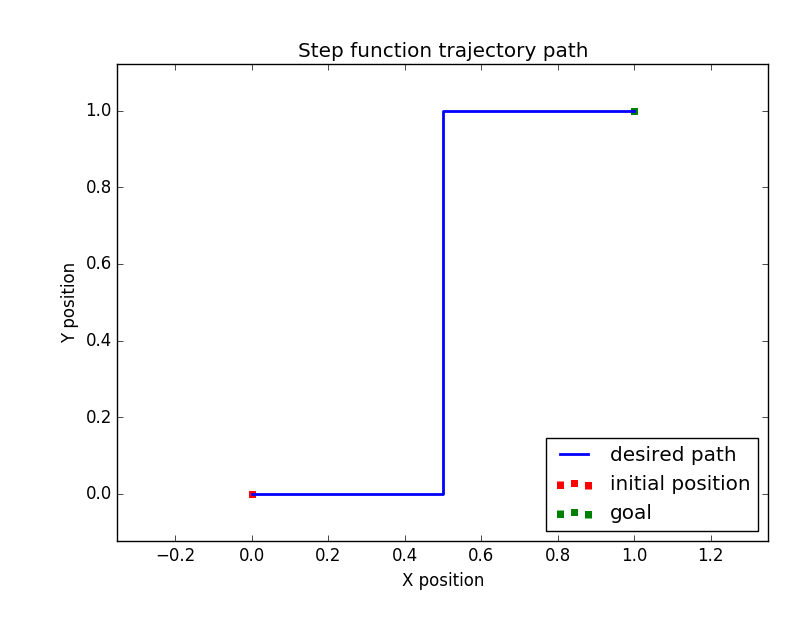
\includegraphics[scale=0.5]{images/step_function.png}
	\caption{Step function trajectory path}
	\label{fig:step_function}
\end{figure}

\subsubsection{Effect of number of basis functions}

Number of basis functions used in the DMP affects the approximation of non-linear forcing function which modifies the shape of motion. More the number of basis functions results into better approximation of forcing function. Better approximation of forcing function means the shape of the trajectory generated by DMP will be more similar to the original trajectory which was used for learning. 

Figure \ref{fig:n_bfs_} illustrates the effect of different number of basis functions on 
learning the trajectory. It can be observed that the increasing the number of basis function results into better approximation of shape the original trajectory.  

The error in mimicking the trajectory is summarized in table \ref{_n_bfs_e}. From data, it can be concluded that the trajectories containing high frequency components can be better approximated with high number of basis functions.

\begin{figure}[H]
	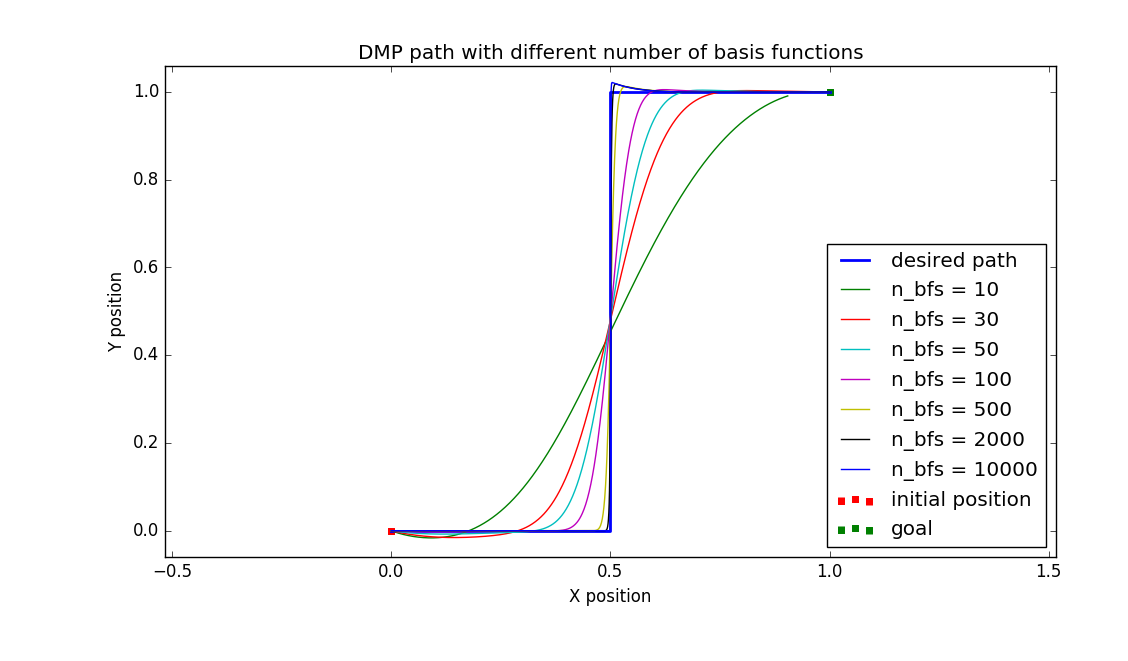
\includegraphics[width=\textwidth]{images/n_bfs_.png}
	\caption{Effect of number of basis functions ($n\_bfs$)}
	\label{fig:n_bfs_}
\end{figure}

\begin{center}
	\begin{table}[H]
		\begin{tabular}{| c | c | c | c | c | c | c | c |}	
			\hline
			Number of basis functions & 10 & 30 & 50 & 100 & 500 & 2000 & 10000\\       
			\hline
			Error & 0.093 & 0.038 & 0.021 & 0.009 & 0.002 & 0.001 & 0.001\\
			\hline
		\end{tabular}
		\caption{Error in mimicking the trajectory}
	\end{table}\label{_n_bfs_e}
\end{center}



Number of basis functions used while learning the DMP also affects the learning of noise. While demonstrating the trajectory, it is possible that high frequency noise is recorded especially because of vibrations and shaking of hands of teacher. If the number of basis function used is very high, high frequency noise is also learned which is not desired. Low number of basis functions result into a smoother trajectory filtering out the noise. 

Use of high number of basis functions also increases the number of computations at run-time as well as at the time of learning the DMP. As the learning algorithm used is linear and DMPs are learned off-line, increase in learning time does not affect much. But if it is required to update the motion command at high frequency while executing the DMP, using high number of basis functions is undesirable.     

\subsubsection{Effect of time step size}   
Motion commands and trajectory generated by DMP framework are in discrete time. Euler's integration method is used to solve the differential equations to obtain the kinematic state at each time step. Hence the choice of step size affects the error in generated trajectory. If the step size used is not small enough, DMP can generate the trajectories those are potentially undesirable and dangerous to be executed by a robot. Large step sizes result in oscillations in the trajectories. Figure \ref{fig:dt_} illustrates the effect of various time step sizes on the trajectories generated by the DMP framework. 

If the step size is not small enough, acceleration at a specific point on the trajectory is not updated for long enough time, so that the generated trajectory overshoots and deviates from the desired trajectory. On next time step, a counter acceleration is applied in order to bring the trajectory close to desired trajectory which again overshoot in opposite direction as previous time step. This intuitive explanation signifies the need of small enough time step for stable behavior of DMP.   


\begin{center}
	\begin{table}[H]
		\centering
		\begin{tabular}{| c | c | c | c | c | c | c | c |}	
			\hline
			Time step size & 0.05 & 0.01 & 0.005 & 0.001 \\       
			\hline
			Error & 0.062 & 0.017 & 0.011 & 0.007 \\
			\hline
		\end{tabular}
		\caption{Error in mimicking the trajectory}
	\end{table}\label{_dt_e}
\end{center}


\begin{figure}[H]
	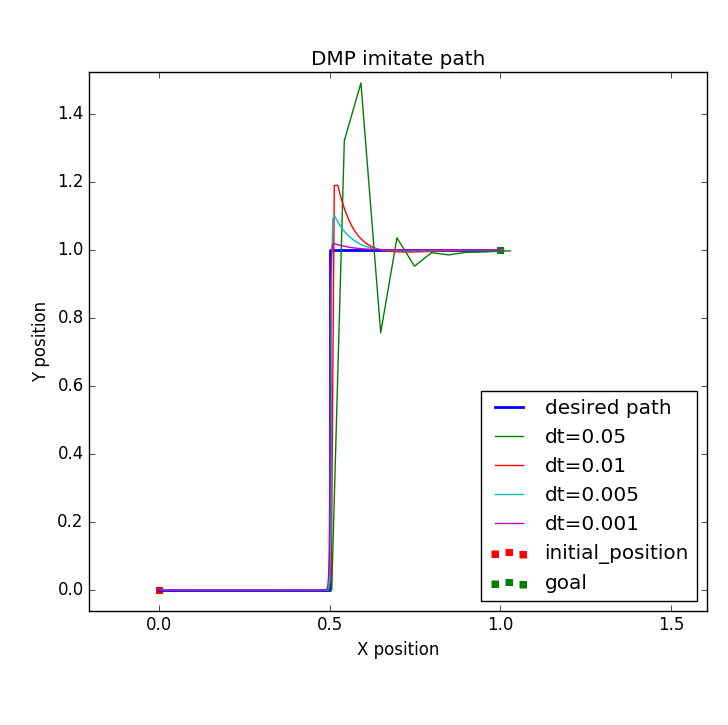
\includegraphics[width=\textwidth]{images/dt_.png}
	\caption{Effect of time step size ($dt$)}
	\label{fig:dt_}
\end{figure}


If the DMP is used for generating instantaneous motion command and feedback form the robot and environment (e.g. position feedback from robot or obstacle from environment) is coupled with DMP, then it is desirable to keep the time step in the order of $10^{-3}$ to avoid large overshoots. 


\subsubsection{Effect of time scaling factor $tau$}   

Time scaling factor ($tau$) is used for modifying the speed of execution of the DMP. It a term which scales the acceleration term produced by transformation system in DMP, which in turn results in scaling of kinematic state at the next step. If the value of $tau$ is set to $1$, then the execution speed of DMP is same as the demonstration. 

If the large value of $tau$ is used, undesirable oscillations can be observed in robot trajectories. The reason behind these oscillations is same as the large time step. The effect of large tau can be nullified by choosing sufficiently small step size. 
\begin{figure}[H]
	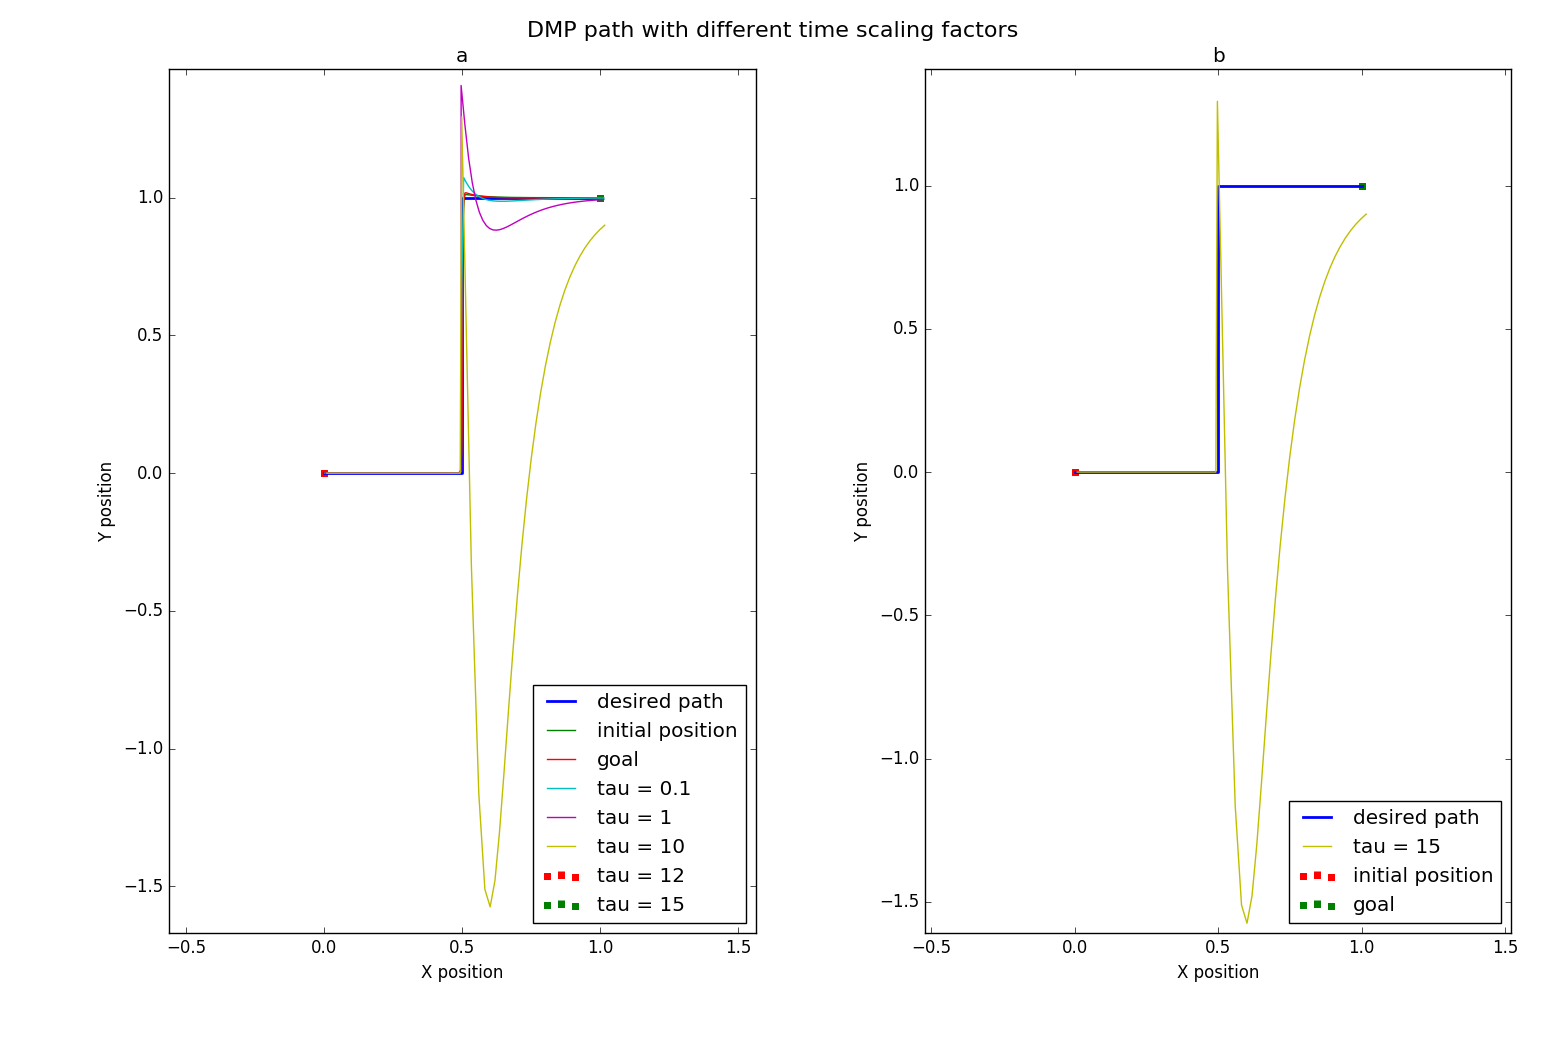
\includegraphics[width=\textwidth]{images/tau_.png}
	\caption{Effect of time scaling factor $tau$}
	\label{fig:tau_}
\end{figure}

\begin{figure}[H]
	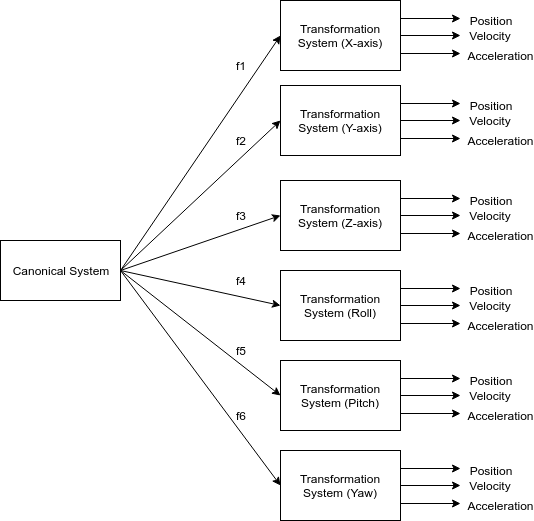
\includegraphics[width=\textwidth]{images/DMP_6DOF.png}
	\caption{6D DMP framework used during experimentation}
	\label{fig:DMP_6DOF}
\end{figure}

\subsection{Learning the Motion Primitive from Demonstrated Trajectories}
\par Learning motion primitive means to learn the weights $w_{i}$ in the eq. \ref{forcing_term}. Above system presented in \cite{ijspeert2013dynamical} is linear in the weights $w_{i}$. So variety of learning algorithms can be used. \cite{ijspeert2013dynamical} uses locally weighted regression to learn the weights. 

Desired behavior that should be exhibited by the system is presented as a tuple ($y_{demo}(t)$, $\dot{y}_{demo}(t)$, $\ddot{y}_{demo}(t)$) representing position, velocity and acceleration respectively where $t = [1,2,3,4,....,p]$. Parameter $g$ is goal hence, $g = y_{demo}(t = p)$ and $y_{0} = y_{demo}(t = 0)$. Parameter $\tau$ is temporal scaling factor which needs to adjusted for achieving desired time scaling in the motion. In order to use LWR for estimating $w_{i}$, eq. (\ref{actual_DMP}) can be rearranged to generate function approximation problem as,
\begin{equation}
f = \ddot{y} - \alpha_{z}(\beta_{z}(g - y) - \dot{y})
\end{equation}
Inserting the information from the demonstrated trajectory in the left-hand side of this equation, we obtain,
\begin{equation}
f_{target} = \ddot{y}_{demo} - \alpha_{z}(\beta_{z}(g - y_{demo}) - \tau\dot{y}_{demo})
\end{equation}

While learning the motion primitives, time scaling factor $\tau$ was set to 1 in all the experiments. 

As we have the values $f_{target}$, we can perform a supervised learning to find a best fit for the function represented by $f_{target}$. 

Locally weighted regression finds for each kernel function $\psi_{i}$ in $f$, the
corresponding $w_{i}$, which minimizes the locally weighted quadratic error criterion,

\begin{equation}
	J_{i} = \sum_{t=1}^{p}\psi_{i}(t)(f_{target}(t)-w_{i}\xi(t))^{2}
\end{equation}

where $\xi_{i} = x(t)(g-y_{0})$ for the discrete system and $\xi_{i} = r$ for rhythmic system. Solution to above linear regression problem is,

\begin{equation}
	w_{i} = \frac{s^{T}\Gamma_{i}f_{target}}{s^{T}\Gamma_{i}s}
\end{equation}

where,\\
\\
\vspace{1cm}
$
s = 
\begin{pmatrix}
\xi(1) \\
\xi(2) \\
\vdots  \\
\xi(p) 
\end{pmatrix}
$
$
\Gamma = 
\begin{pmatrix}
	\psi_{i}(1) &   &  & 0 \\
	 &\psi_{i}(2)&  &  \\
	 &  & \ddots &   \\
	0 &  &  & \psi_{i}(p)
\end{pmatrix}
$
$
f_{target} = 
\begin{pmatrix}
f_{target}(1) \\
f_{target}(2) \\
\vdots  \\
f_{target}(p) 
\end{pmatrix}
$


 

After 

 




\subsection{Inverse Kinematics Solver and Trajectory Controller}

In order to execute the task-space trajectory generated by DMP framework, Cartesian velocities are needed to be converted to the joint velocities with the help of inverse kinematic solver. Robot arm used in the experiments (KUKA YouBot arm) has five degrees of freedom. Five degrees of freedom are not sufficient to carry out 6 degrees of freedom cartesian motion. Due to this design deficiency, manipulator is always in the singular configuration. It is well-known that when a manipulator is at-or is in the neighborhood of a singular configuration, severe restrictions may occur on its motion. To overcome this situation, \textit{weighted damped least square pseudo inverse method} for computing joint velocities was chosen. This method allows us to loose the constraints on individual degrees of freedom in task-space. Which allowed us to ignore velocity constraints on 3 rotational degrees of freedom. This is called user-defined accuracy method to control the manipulator. \cite{chiaverini1994review}
\\
The relation between joint space and task space velocity can be given by, 

\begin{equation}\label{theta_dot}
	v = J(\theta) \dot{\theta} 
\end{equation}

\begin{equation}
	\dot{\theta} = J(\theta)^{-1}  v
\end{equation} 
Where, \\
$J(\theta)$ is jacobian of manipulator, \\
$v$ is task space velocity vector, \\
$\dot{\theta}$ is joint space velocity vector. \\

When manipulator is near a singularity, sigma  large joint velocities may occur or degenerate directions may exist where end-effector velocity
is not feasible\cite{chiaverini1994review}. To overcome this situation, damped least square method can be used where a degraded solution is generated near the singularities proposed in \cite{wampler1986manipulator, nakamura1986inverse}.  

\begin{equation}
	J^{T}(\theta)v = (J^{T}(\theta)J(\theta) + \lambda ^{2}I)\dot{\theta}
\end{equation}

Where, \\
$\lambda > 0 $ is the damping factor, and \\
$I $ is identity matrix. \\

Solution to above problem can be given by, 
\begin{equation}\label{damped_least_sol}
	\dot{\theta} = (J^{T}(\theta)J(\theta) + \lambda^{2}I)^{-1}J^{T}(\theta)v
\end{equation} 

It should be noted that, if the value of $\lambda$ in eq. \ref{damped_least_sol} is set to 0, eq. \ref{damped_least_sol} reduces to eq. \ref{theta_dot}.

The effect of value of lambda on joint velocities can be analyzed in detail by singular value decomposition of the Jacobian matrix and that is, 

\begin{equation}
	J = \sum_{i=1}^{6}\sigma_{i}u_{i}\textbf{v}_{i}^{T}
\end{equation} 

Using singular value decomposition, equation \ref{damped_least_sol} can be re-written as,

\begin{equation}
\dot{\theta} = \sum_{i=1}^{6}\frac{\sigma_{i}}{\sigma_{i}^{2} + \lambda^{2} }\sigma_{i}u_{i}\textbf{v}_{i}^{T}v
\end{equation} 

It can be observed in above equation that if $\sigma \gg \lambda$, then $\lambda$ has practically no effect on joint velocities. But if $\sigma$ is close to zero, then the joint velocities are greatly affected by value of $\lambda$.  

Since the arm has only five degrees of freedom, it is always in singular configuration and hence it is not possible to execute the 6 degrees of motion at all the time instances. This situation can be overcome by ignoring motion in 3 rotational degrees of freedom with the help of the method called \textit{weighted damped least square pseudo inverse}. In this method, 	
\section{Setup}


\section{Experimental Design}
